

\tikzset{%
  client/.style={
    rectangle,
    thick,
    draw,
    minimum size=0.7cm,
    text width=1cm,
    align=center
  },
  client missing/.style={
    draw=none, 
    scale=2,
    text height=0.333cm,
    execute at begin node=$\cdots$
  },
}


\begin{document}

%----------------------------------------------------------------------------------------
%	TITLE PAGE
%----------------------------------------------------------------------------------------

\title[联邦学习]{\huge{联邦学习中的优化问题}  \\
\medskip
\small{Optimizations in Federated Learning}
} % The short title appears at the bottom of every slide, the full title is only on the title page

% \author[文豪]{文豪} % Your name

% \institute[北京航空航天大学] % Your institution as it will appear on the bottom of every slide, may be shorthand to save space
% {
% 数学科学学院 \\ % Your institution for the title page
% \medskip
% \textit{wenh06@gmail.com} % Your email address
% 北京航空航天大学 \\
% 数学科学学院 \qquad 北京航空航天大学
% }

% \logo{\includegraphics[height=1.5cm]{logo}}
% \logoii{\includegraphics[height=1cm]{logo2}}

% \date{\footnotesize 2021年4月13日} % Date, can be changed to a custom date

\setlength{\belowdisplayskip}{5pt} \setlength{\belowdisplayshortskip}{5pt}
\setlength{\abovedisplayskip}{5pt} \setlength{\abovedisplayshortskip}{5pt}

%------------------------------------------------

\begin{frame}
\titlepage % Print the title page as the first slide
\end{frame}

%------------------------------------------------

\begin{frame}
% \frametitle{Overview} % Table of contents slide, comment this block out to remove it
\tableofcontents % Throughout your presentation, if you choose to use \section{} and \subsection{} commands, these will automatically be printed on this slide as an overview of your presentation
\end{frame}

%------------------------------------------------

%------------------------------------------------
%	PRESENTATION SLIDES
%------------------------------------------------


% PPT version (read only share link): https://www.kdocs.cn/l/cigmbsd3uAI4


%------------------------------------------------

\section{引言}

%------------------------------------------------
% Page 1

\begin{frame}
\frametitle{引言}

联邦学习(Federated Learning)来源于机器(深度)学习模型分布式(Distributed)训练的需求

\begin{figure}
    \centering
    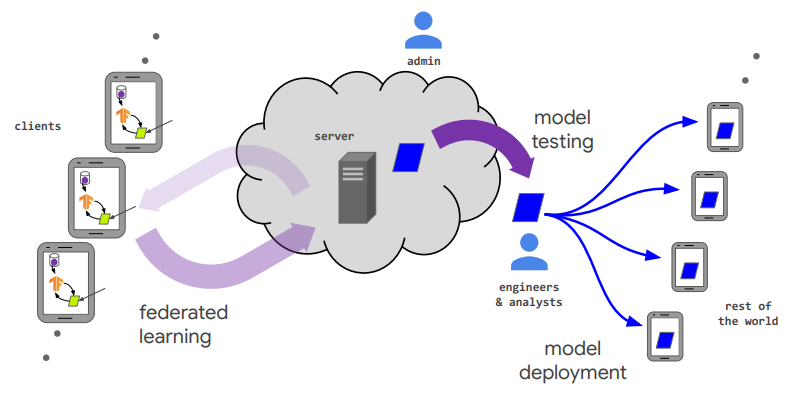
\includegraphics[width=\textwidth,keepaspectratio]{images/fl_overview.png}
\end{figure}

{\footnotesize
图片来源:Kairouz et al., Advances and open problems in federated learning, 2019
}

\end{frame}

%------------------------------------------------
% Page 15

\begin{frame}
\frametitle{引言}

Federated Learning这个名词首次由Google的研究人员McMahan等人在文章 \emph{Communication-Efficient Learning of Deep Networks from Decentralized Data} (2017)  中提出。

\vspace{3em}
\pause

相关的分布式的模型训练(优化)方法则可以追溯到更早的时间,例如Boyd等人的 \emph{Distributed Optimization and Statistical Learning via the Alternating Direction Method of Multipliers} (2010)

\end{frame}

%------------------------------------------------
% Page 15

\begin{frame}
\frametitle{联邦学习研究的一些核心的问题}

\begin{itemize}
    \item {\Large\bfseries EE (Efficiency \& Effectiveness)}
    \begin{itemize}
        \item[$\bullet$] {\large\bfseries Optimization}
        \vspace{0.5em}
        \pause
        {\pgfsetfillopacity{0.4} \footnotesize
        \item[$\bullet$] Compression
        }
    \end{itemize}
    \vspace{1em}
    {\pgfsetfillopacity{0.4} \footnotesize
    \item Privacy \& Security
    \begin{itemize}
        \item[$\bullet$] Differential Privacy (DP)
        \item[$\bullet$] Secure Multi-Party Computing (SMPC)
        \item[$\bullet$] Trusted Execution Environment (TEE)
        \item[$\bullet$] Homomorphic Encryption (HE)
    \end{itemize}
    \item Applications
    \begin{itemize}
        \item[$\bullet$] Medical
        \item[$\bullet$] Recommendation
        \item[$\bullet$] Finance
    \end{itemize}
    \item $\cdots\cdots$
    }
\end{itemize}

\end{frame}

%------------------------------------------------

\section[联邦学习中的优化]{联邦学习中的优化问题与算法}

%------------------------------------------------
% Page 15

\begin{frame}
\frametitle{问题描述}

一般来说,联邦学习中我们考虑的是如下的优化问题
\begin{align*}
    & \text{minimize} \quad f(x) = \expectation\limits_{i \sim {\mathcal{P}}} [f_i(x)] \\
    & \text{where} \quad f_i(x) = \expectation\limits_{z \sim \mathcal{D}_i} [\ell_i(x; z)]
\end{align*}
这里的$\mathcal{P}$为``client''的分布,$\mathcal{D}_i$为``client'' i 的数据分布,$\ell_i$为损失函数。

\pause
\vspace{1em}

或者更简单地,考虑如下的优化问题
\begin{align*}
    & \text{minimize} \quad f(x) = \dfrac{1}{N} \sum\limits_{i=1}^N f_i(x)
\end{align*}

\end{frame}

%------------------------------------------------
% Page 15

\begin{frame}
\frametitle{问题描述}

这里的``client''是广义上的``client'',涵盖很多场景,例如
\begin{itemize}
    \item (多个机器上的)多张显卡
    % 这种情况下,数据来源(分布)可能是相同的(例如都是ImageNet),但是partition是固定的,需要区别于 datacenter 的情况
    \item 多个移动设备
    % 这种情况下,数据来源一般是不同的
\end{itemize}

\pause
\vspace{1.5em}

前者一般被称作cross-silo,后者一般被称作cross-device。在cross-device的场景下,一般来说,通信效率才是整个系统的瓶颈所在,此外还要考虑掉队者(straggler)等问题需要考虑。

\end{frame}

%------------------------------------------------
% Page 15

\begin{frame}
\frametitle{数据分布}

在真实场景下,各个client的分布$\mathcal{D}_i$一般不是独立同分布的(non-IID, 或称heterogeneous)。non-IID数据分布下,算法的收敛性分析相比IID数据下要更加困难,需要更多额外的假设,对client之间的数据分布的不同性(dissimilarity)进行定量上的限制。

\vspace{1.5em}

一般地,这种限制以gradient variance给出,例如bounded inter-client gradient variance (BCGV):
$$\expectation\limits_{i \sim {\mathcal{P}}} \lVert \nabla f_i(x) - \nabla f(x) \rVert_2^2 \leqslant \text{const} \quad \text{ for all } x$$

\end{frame}

%------------------------------------------------
% Page 15

\begin{frame}
\frametitle{联邦学习的一般性框架(流程)}

\begin{itemize}
    \item client selection
    \item parameter broadcast
    \item {\bfseries client computation (local parameter update)}
    \item parameter aggregation
    \item {\bfseries server computation (global parameter update)}
\end{itemize}

\end{frame}

%------------------------------------------------
% Page 15

% reference: FLOW - Adaptive Federated Optimization

\begin{frame}
\frametitle{联邦学习的一般性框架(流程)}

Broadcast and local update:

\vspace{2em}

\begin{figure}
\centering
\begin{tikzpicture}[]
\node[] (slide-center) {};
\node[client, above=3em of slide-center] (server) {server $x$};
\node[client, below left = 1.5cm and 3.5cm of server.south] (client-1) {client $x_1$};
\node[client, right = 0.4cm of client-1.east] (client-2) {client $x_2$};
\node[client, right = 0.4cm of client-2.east] (client-3) {client $x_3$};
\node[client missing, right = 0.1cm of client-3.east] (client-missing) {};
\node[client, right = 0.1cm of client-missing.east] (client-n) {client $x_n$};
\path[->] ([xshift=-0.5cm,yshift=-0.1cm]server.south) edge ([yshift=0.15cm]client-1.north);
\path[->] ([xshift=-0.2cm,yshift=-0.1cm]server.south) edge ([yshift=0.15cm]client-2.north);
\path[->] ([xshift=0.05cm,yshift=-0.1cm]server.south) edge ([yshift=0.15cm]client-3.north);
\path[->] ([xshift=0.4cm,yshift=-0.1cm]server.south) edge ([yshift=0.15cm]client-n.north);
\node[text width=1.2cm, align=center, right=0.3cm of client-n.east] (local-update) {local update};
\node[text width=1.8cm, align=center, above left=0.5cm and 0.3cm of local-update.north] () {params broadcast};
\end{tikzpicture}
\end{figure}

\end{frame}

%------------------------------------------------
% Page 15

% reference: FLOW - Adaptive Federated Optimization

\begin{frame}
\frametitle{联邦学习的一般性框架(流程)}

Aggregate and global update:

\vspace{2em}

\begin{figure}
\centering
\begin{tikzpicture}[]
\node[] (slide-center) {};
\node[client, above=3em of slide-center] (server) {server $x$};
\node[client, below left = 1.5cm and 3.5cm of server.south] (client-1) {client $x_1$};
\node[client, right = 0.4cm of client-1.east] (client-2) {client $x_2$};
\node[client, right = 0.4cm of client-2.east] (client-3) {client $x_3$};
\node[client missing, right = 0.1cm of client-3.east] (client-missing) {};
\node[client, right = 0.1cm of client-missing.east] (client-n) {client $x_n$};
\path[->] ([yshift=0.15cm]client-1.north) edge ([xshift=-0.5cm,yshift=-0.1cm]server.south);
\path[->] ([yshift=0.15cm]client-2.north) edge ([xshift=-0.2cm,yshift=-0.1cm]server.south);
\path[->] ([yshift=0.15cm]client-3.north) edge ([xshift=0.05cm,yshift=-0.1cm]server.south);
\path[->] ([yshift=0.15cm]client-n.north) edge ([xshift=0.4cm,yshift=-0.1cm]server.south);
\node[text width=1.2cm, align=center, right=0.3cm of server.east] (global-update) {global update};
\node[text width=1.8cm, align=center, below right=0.25cm and 0.3cm of global-update.south] () {aggregation};
\end{tikzpicture}
\end{figure}

\end{frame}

%------------------------------------------------

\section{FedOpt}

%------------------------------------------------
% Page 15

\begin{frame}
\frametitle{从FedAvg到FedOpt}

Google研究人员McMahan等人。。。。(待写)

\end{frame}

%------------------------------------------------
% Page 15

\begin{frame}
\frametitle{FedSGD -- baseline}

\begin{figure}
\centering
\begin{tikzpicture}[]
\node[] (slide-center) {};
\node[left=9cm of slide-center] (x_t) {$x_t$};
\node[above right = 1.5cm and 0.6cm of x_t] (x_1_0) {$x_{1,t}^0$};
\node[below = 0.6cm of x_1_0] (x_2_0) {$x_{2,t}^0$};
\node[below = 0.4cm of x_2_0] (missing) {$\vdots$};
\node[below = 0.4cm of missing] (x_n_0) {$x_{n,t}^0$};
\foreach \m in {1,2,n}
{
    \path[->,brown] (x_t) edge (x_\m_0);
}

\foreach \m in {1,2,n}
{
    \node[right = 0.6cm of x_\m_0] (x_\m_1) {$x_{\m,t}^1$};
    \path[->] (x_\m_0) edge (x_\m_1);
}
\node[below right = 1.5cm and 0.6cm of x_1_1] (x_t_1) {$x_{t+1}$};
\foreach \m in {1,2,n}
{
    \path[->,green] (x_\m_1) edge (x_t_1);
}
\draw[dashed,red,thick] ([xshift=-0.7cm,yshift=0.1cm]x_1_0.north) rectangle ([xshift=0.7cm,yshift=-0.1cm]x_n_1.south);
\node[below right=0.3cm and -0.5cm of x_n_0.south] () {ONE local step};

\node[above right = 1.5cm and 0.6cm of x_t_1] (x_11_0) {$x_{1,t+1}^0$};
\node[below = 0.6cm of x_11_0] (x_12_0) {$x_{2,t+1}^0$};
\node[below = 0.4cm of x_12_0] (missing1) {$\vdots$};
\node[below = 0.4cm of missing1] (x_1n_0) {$x_{n,t+1}^0$};
\foreach \m in {1,2,n}
{
    \path[->,brown] (x_t_1) edge (x_1\m_0);
}

\foreach \m in {1,2,n}
{
    \node[right = 0.6cm of x_1\m_0] (x_1\m_1) {$x_{\m,t+1}^1$};
    \path[->] (x_1\m_0) edge (x_1\m_1);
}
\node[below right = 1.5cm and 0.6cm of x_11_1] (x_t_2) {$x_{t+2}$};
\foreach \m in {1,2,n}
{
    \path[->,green] (x_1\m_1) edge (x_t_2);
}
\draw[dashed,red,thick] ([xshift=-0.8cm,yshift=0.1cm]x_11_0.north) rectangle ([xshift=0.8cm,yshift=-0.1cm]x_1n_1.south);
\node[below right=0.3cm and -0.5cm of x_1n_0.south] () {ONE local step};
\end{tikzpicture}
\end{figure}

\end{frame}

%------------------------------------------------
% Page 15

\begin{frame}
\frametitle{FedAvg}

\begin{figure}
\centering
\begin{tikzpicture}[]
\node[] (slide-center) {};
\node[left=9cm of slide-center] (x_t) {$x_t$};
\node[above right = 1.5cm and 0.8cm of x_t] (x_1_0) {$x_{1,t}^0$};
\node[below = 0.6cm of x_1_0] (x_2_0) {$x_{2,t}^0$};
\node[below = 0.4cm of x_2_0] (missing) {$\vdots$};
\node[below = 0.4cm of missing] (x_n_0) {$x_{n,t}^0$};
\foreach \m in {1,2,n}
{
    \path[->,brown] (x_t) edge (x_\m_0);
}

\foreach \m in {1,2,n}
{
    \node[right = 0.8cm of x_\m_0] (x_\m_1) {$x_{\m,t}^1$};
    \path[->] (x_\m_0) edge (x_\m_1);
}
\foreach \m in {1,2,n}
{
    \node[right = 0.8cm of x_\m_1] (x_\m_2) {$x_{\m,t}^2$};
    \path[->] (x_\m_1) edge (x_\m_2);
}
\foreach \m in {1,2,n}
{
    \node[right = 0.5cm of x_\m_2] (missing_\m) {$\cdots$};
    \path[->] (x_\m_2) edge (missing_\m);
}
\foreach \m in {1,2,n}
{
    \node[right = 0.5cm of missing_\m] (x_\m_K) {$x_{\m,t}^K$};
    \path[->] (missing_\m) edge (x_\m_K);
}
\node[below right = 1.5cm and 0.8cm of x_1_K] (x_t_1) {$x_{t+1}$};
\foreach \m in {1,2,n}
{
    \path[->,green] (x_\m_K) edge (x_t_1);
}
\draw[dashed,red,thick] ([xshift=-0.7cm,yshift=0.1cm]x_1_0.north) rectangle ([xshift=0.8cm,yshift=-0.1cm]x_n_K.south);
\node[below=0.3cm of x_n_2] () {$K$ local steps};
\end{tikzpicture}
\end{figure}

\end{frame}

%------------------------------------------------
% Page 15

\begin{frame}
\frametitle{收敛性}



\end{frame}

%------------------------------------------------

\section{ADMM}

%------------------------------------------------
% Page 15

\begin{frame}
\frametitle{GADMM}



\end{frame}

%------------------------------------------------
% Page 15

\begin{frame}
\frametitle{CQ-GGADMM}



\end{frame}

%------------------------------------------------
% Page 15

\begin{frame}
\frametitle{收敛性}



\end{frame}

%------------------------------------------------
% Page 15

\begin{frame}
\frametitle{参考文献}



\end{frame}


%------------------------------------------------

% \begin{frame}

% \Huge{\centerline{\bfseries The End}}

% \vspace{0.5em}

% \Huge{\centerline{\phantom{a}\bfseries 谢谢!}}

% \end{frame}

%------------------------------------------------

\end{document}
